\documentclass{article}

\usepackage{graphicx,natbib,amsmath,hyperref}

\title{Errorchrons and anchored isochrons in IsoplotR}

\author{Pieter Vermeesch\\
  Department of Earth Sciences\\
  University College London\\
  Gower Street\\
  London WC1E 6BT\\
  United Kingdom
}

\begin{document}

\maketitle

\begin{abstract}
  Isochrons are usually fitted by `York regression', which uses a
  weighted least squares approach that accounts for correlated
  uncertainties in both variables. Despite its tremendous popularity
  in modern geochronology, the York algorithm has two important
  limitations that reduce its utility in several applications. First,
  it does not provide a satisfactory mechanism to deal with so-called
  `errorchrons', i.e. datasets that are overdispersed with respect to
  the analytical uncertainties. Second, York regression is not readily
  amenable to anchoring, in which either the slope or the intercept of
  the isochron is fixed based on some external information. Anchored
  isochrons can be very useful in cases where the data are
  insufficiently spread out to constrain both the radiogenic and
  non-radiogenic isotopic composition.

  This paper addresses both of these issues by extending a maximum
  likelihood algorithm that was first proposed by Titterington and
  Halliday (1979, Chemical Geology 26.3-4: 183-195). The new algorithm
  offers the ability to attribute any excess dispersion to either the
  inherited component (`model~3a') or to diachronous closure of the
  isotopic system (`model~3b'). It provides an opportunity to anchor
  isochrons either to a fixed nonradiogenic composition or a fixed
  age. Last but not least, it allows the user to attach meaningful
  analytical uncertainty to the anchor. The new method has been
  implemented in IsoplotR for immediate use in Ar/Ar, Pb/Pb, U/Pb,
  Th/Pb, Rb/Sr, Sm/Nd, Lu/Hf, Re/Os, K/Ca and U-Th-He geochronology.
\end{abstract}

\section{Introduction}\label{sec:intro}

  Isochrons are mixing lines between radiogenic and inherited isotopic
  endmembers. They are an essential component of radiometric
  geochronology and exist in several
  forms. Sections~\ref{sec:intro}--\ref{sec:anchorerr} of this paper
  will deal with the simple case of `P/D-isochrons', which apply to
  geochronometers that are based on the decay of a single radioactive
  parent nuclide ($P$; e.g., ${}^{87}$Rb, ${}^{40}$K, ${}^{147}$Sm) to
  a particular daughter nuclide ($D$; e.g., ${}^{87}$Sr, ${}^{40}$Ar,
  ${}^{143}$Nd). Sections~\ref{sec:PbPb} and \ref{sec:UPb} will
  discuss Pb/Pb- and U/Pb-isochrons, respectively.  These are based on
  the paired decay of two parents (${}^{238}$U and ${}^{235}$U) to two
  daughters (${}^{206}$Pb and ${}^{207}$Pb, respectively) and require
  linear regression in two or three dimensions.\medskip

  P/D-isochrons come in two types. `Conventional' isochrons are
  straight line relationships of the following kind:
  \begin{equation}
    \left[\frac{D}{d}\right]_i =
    \left[\frac{D}{d}\right]_0 +
    \left[\frac{P}{d}\right]_i \left(e^{\lambda{t}}-1\right)
    \label{eq:conventionalPD}
  \end{equation}

  \noindent where $i$ is the aliquot number ($1\leq{i}\leq{n}$), $d$
  is a non-radiogenic sister isotope of $D$, $[D/d]_0$ is the
  inherited component, $\lambda$ is the decay constant and $t$ is the
  time elapsed since isotopic closure. A full list of definitions is
  provided in Appendix~\ref{app:definitions}. `Inverse' isochrons are
  obtained by permuting $P$, $D$ and $d$:
  \begin{equation}
    \left[\frac{d}{D}\right]_i =
    \left[\frac{d}{D}\right]_0
    \left\{
    1 - \left[\frac{P}{D}\right]_i \left(e^{\lambda{t}}-1\right)
    \right\}
    \label{eq:inversePD}
  \end{equation}

  The choice between conventional and inverse isochrons depends on the
  relative precision of the mass spectrometer measurements.  Inverse
  isochrons are preferred if $d\ll{D}$. Otherwise, conventional
  isochrons are fine \citep{li2021}.\medskip

  Equations~\ref{eq:conventionalPD} and \ref{eq:inversePD} can be
  recast into a generic linear form:
  \begin{equation}
    y_i = a + b x_i
    \label{eq:yabx}
  \end{equation}

  Table~\ref{tab:PDDD} maps the parameters of this generic equation to
  the parameters of Equations~\ref{eq:conventionalPD},
  \ref{eq:inversePD} and subsequent variants thereof.
  Equation~\ref{eq:yabx} is usually solved by \citet{york2004}
  regression (hereafter simply referred to as `York regression').
  York regression uses a least squares algorithm to estimate the
  intercept ($a$) and slope ($b$) of the isochron line from an
  $n\times{5}$ table of paired isotopic ratio measurements, their
  standard errors and their error
  correlations.\medskip

  Although this paper will use the York parameters $a$ and $b$ to fit
  the isochron, all results will be presented in terms of the
  geologically more meaningful inherited endmember ratio $[D/d]_0$ and
  radiogenic endmember ratio $[D/P]^\ast\equiv{e}^{\lambda{t}}-1$,
  where $[D/d]_0=a$ and $[D/P]^\ast=b$ for conventional isochrons, and
  $[D/d]_0=1/a$ and $[D/P]^\ast=-b/a$ for inverse isochrons
  \citep{li2021}.\medskip

  The most accurate and precise results are obtained from samples that
  are evenly spread along the isochron line, spanning the entire range
  of values from the inherited to the radiogenic
  endmember. Unfortunately, this condition is not always fulfilled. It
  is not uncommon for most or all aliquots in a sample to cluster
  together at one point along the isochron, making it difficult to
  accurately estimate the endmember compositions. For example, no
  precise isochron ages can be obtained from samples whose radiogenic
  daughter component is dwarfed by the inherited daughter
  component. Conversely, the composition of the inherited component
  cannot be precisely estimated in extremely radiogenic samples.
  Finally, when the data cluster together in the middle, then neither
  endmember component can be reliably determined
  (Figure~\ref{fig:cluster}).\medskip
  
  Sometimes, such poorly constrained isochrons can be fixed using
  external information. For example, if the composition of the
  inherited component is known through some independent means (e.g.,
  by analysing a cogenetic mineral that is naturally poor in $P$ and
  rich in $D$ and $d$), then this information can be used to anchor
  the isochron. Anchoring reduces the number of unknown parameters by
  one, benefitting numerical stability and precision. Conversely, if
  the age of the sample is known, then the inherited component can be
  estimated by anchoring to the radiogenic endmember.\medskip

  There currently exists no formally documented way to anchor York
  regression.  A commonly used `hack' is to add an extra data point
  with infinite precision representing either the inherited or
  radiogenic endmember component. However, this hack does not provide
  a satisfactory mechanism to assign uncertainty to the anchor. This
  paper solves that problem. Section~\ref{sec:MLyork} introduces a
  maximum likelihood formulation of York regression, which is amenable
  to anchoring with uncertainty. Section~\ref{sec:overdispersion}
  shows how this formulation can be used to model `errorchrons' that
  are overdispersed with respect to the analytical
  uncertainties.\medskip

  Section~\ref{sec:specific} provides further details about the
  implementation of maximum likelihood regression, which can attribute
  overdispersion to either the intercept (`model~3a') or slope
  (`model~3b') of the linear fit. It turns out that model~3b is
  computationally more challenging than
  model~3a. Section~\ref{sec:flipper} shows how this issue can be
  avoided by inverting and flipping the isochron axes.\medskip

  Section~\ref{sec:anchor} shows how anchored isochron regression
  represents a trivial special case of the maximum likelihood
  algorithm. Section~\ref{sec:anchorerr} attaches two different
  geological interpretations to the uncertainty of isochron
  anchors. These two interpretations lead to two different fit models
  (`model~1' and `model~3', which are so named for historical
  reasons). Sections~\ref{sec:PbPb} and \ref{sec:UPb} apply the same
  logic to Pb/Pb and U/Pb isochrons, respectively.  Finally,
  Section~\ref{sec:IsoplotR} shows how the new algorithms can be used
  within the \texttt{IsoplotR} software package.
  
  \begin{figure}[!ht]
    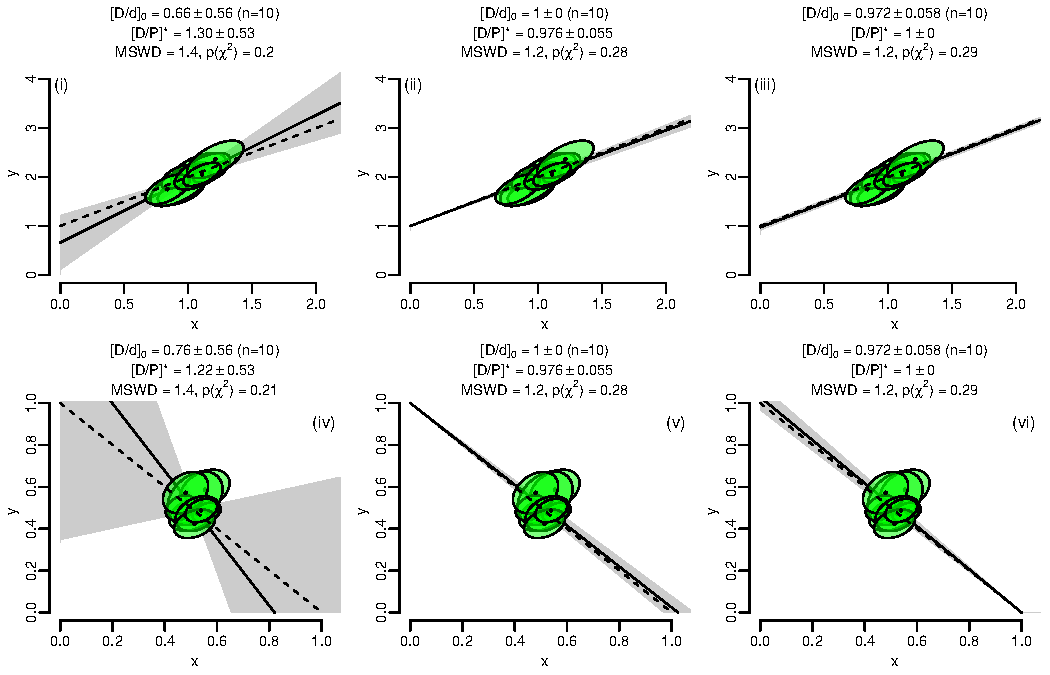
\includegraphics[width=15cm]{fig1.pdf}
    \caption{P/D-isochron diagrams for a synthetic dataset generated
      using the procedures of Appendix~\ref{app:syntheticdata}. The
      true slope and intercept are $a=1$ and $b=1$ for the
      conventional isochrons (i--iii), and $a=1$ and $b=-1$ for the
      inverse isochrons (iv--vi). These parameter values correspond to
      $[D/d]_0=[D/P]^{\ast}=1$. The true trends are shown as dashed
      lines and the estimated trends as solid lines, with 95\%
      confidence envelopes shown in grey. The estimated parameter
      values are shown above the panels. Unconstrained isochron
      regression (i and iv) yields imprecise and inaccurate
      results. Fixing the inherited component (ii and v) or the
      radiogenic component (iii and vi) greatly improves both aspects
      of the fit.}
    \label{fig:cluster}
  \end{figure}
  
\section{Maximum likelihood formulation of York regression}\label{sec:MLyork}

\citet{york2004} use the method of least squares to fit the general
problem of weighted regression with correlated uncertainties in both
variables. \citet{titterington1979} obtained identical results using
the method of maximum likelihood. The latter approach offers greater
flexibility than least squares and will be used in the remainder of
this paper.\medskip

The method of maximum likelihood is a standard statistical technique
to estimate the parameters of a probability distribution from a set of
measurements. In the case of two-dimensional isochron regression, the
parameters are the intercept $a$, the slope $b$ and the true (but
unknown) $x_i$-values. The data are the $X_i$ and $Y_i$-measurements
along with their assumed uncertainties and error correlations (see
Appendix~\ref{app:definitions} for a full list of definitions). For a
dataset of $n$ aliquots, there are $2n$ measurements ($n$ $X_i$-values
and $n$ $Y_i$-values) and $n+2$ parameters ($a$, $b$ and $n$
$x_i$-values). That leaves $2n-n-2=n-2$ `degrees of freedom' to
estimate the parameters.\medskip

This overconstrained problem can be solved by minimising the paired
differences (`residuals') between the true $x_i$- and $y_i$-values
(where $y_i = a + b x_i$) and the measured $X_i$- and $Y_i$-values:
\begin{equation}
  \begin{cases}
    X_i = x_i + \epsilon_{x,i} \\
    Y_i = a + b x_i + \epsilon_{y,i}
  \end{cases}
  \label{eq:model1}
\end{equation}

To make the problem tractable, the vector of residuals
$\mathbf{\Delta}_i$ is assumed to be drawn from a bivariate normal
distribution with zero mean and covariance matrix $\mathbf{\Sigma}_i$:
\begin{equation}
  \mathbf{\Delta}_i \equiv
  \left[
    \begin{array}{@{}c@{}}
      X_i - x_i\\
      Y_i - y_i
    \end{array}
    \right]
  =
  \left[
    \begin{array}{@{}c@{}}
      \epsilon_{x,i}\\
      \epsilon_{y,i} 
    \end{array}
    \right]
  \mbox{~and~}
  \mathbf{\Sigma}_i \equiv
  \left[
    \begin{array}{@{}c@{~}c@{}}
      s[X_i]^2 & s[X_i,Y_i]\\
      s[X_i,Y_i] & s[Y_i]^2
    \end{array}
    \right].
  \label{eq:model1DEi}
\end{equation}

The product of the normal probabilities for all the aliquots (from
$1\leq{i}\leq{n}$) is called the `likelihood' of the parameters given
the data. Maximising this number produces the most accurate possible
parameter estimates $\hat{a}$, $\hat{b}$ and
$\hat{x}_i$. Alternatively, and equivalently, the same estimates can
be obtained by maximising the logarithm of the likelihood.  This is
the preferred approach as it improves numerical stability and
facilitates the estimation of the parameter uncertainties. The
log-likelihood function can be formally defined as:
\begin{equation}
  \mathcal{LL}(\mbox{parameters}|\mbox{data}) =
  - \frac{1}{2}
  \sum\limits_{i=1}^{n} \left( 2\pi +
  \ln|\mathbf{\Sigma}_i| +
  \mathbf{\Delta}_i^T \mathbf{\Sigma}_i^{-1} \mathbf{\Delta}_i \right)
  \label{eq:LL}
\end{equation}

This formulation allows for correlated uncertainties between the
variables ($s[X_i,Y_i]\neq{0}$ in Equation~\ref{eq:model1DEi}), but
not between aliquots ($s[X_i,Y_j]={0}$ if
${i}\neq{j}$). \citet{daeron2023} discuss the generalised case of
`omnivariant' regression, where this requirement has been relaxed and
Equation~\ref{eq:LL} is replaced with a single matrix expression.

\section{Dealing with overdispersion}\label{sec:overdispersion}

The degree to which the residuals $\mathbf{\Delta}_i$ are consistent
with the assumed analytical uncertainties $\mathbf{\Sigma}_i$ can be
assessed using a Chi-square test and MSWD parameter. Readers who are
not familiar with these concepts are referred to Appendix~\ref{app:X2}
for details. Isochrons that exhibit significant overdispersion with
respect to the analytical uncertainties are colloquially referred to
as `errorchrons'. Whether it is right to use such a pejorative term
for this common phenomenon is debatable \citep{schaen2021}.  Four
approaches may be used to deal with errorchrons:

\begin{description}
\item{\textbf{model~1}:} Inflate the analytical uncertainties by a
  factor $\sqrt{\mbox{MSWD}}$.
\item{\textbf{model~2}:} Ignore the analytical uncertainties and
  replace York regression with orthogonal regression or a similar
  technique. This approach will not be discussed further in this
  paper.
\item{\textbf{model~3}:} Quantify the dispersion as an additional free
  parameter. There are two options for doing so:
  \begin{description}
  \item{\textbf{model~3a}:} Attribute the excess dispersion to
    variability of the inherited component and, hence, the isochron
    intercept. For conventional isochrons, this means that the true
    isotopic ratios of the cogenetic aliquots do not belong to a
    single isochron line, but to a family of parallel isochron lines
    whose intercepts are normally distributed
    \citep{titterington1979}. The standard deviation of this normal
    distribution ($\sigma_a$) can be used to quantify the dispersion
    of the data around the `central' isochron line.
  \item{\textbf{model~3b}:} Attribute the excess dispersion to
    diachronous closure of the isotopic system. This mechanism
    produces families of conventional isochrons that share a common
    intercept but differ in their slopes. Again, the distribution of
    the slopes can be assumed to follow a normal distribution, with
    mean $b$ and standard deviation $\sigma_b$. The latter value can
    be used to quantify the dispersion of the data, which in this case
    captures the degree of diachroneity.
  \end{description}
\end{description}

Model~3a isochron regression can be formalised by modifying
Equation~\ref{eq:model1} as follows:
\begin{equation}
  \begin{cases}
    X_i = x_i + \epsilon_{x,i} \\
    Y_i = a + b x_i + \epsilon_a + \epsilon_{y,i}
  \end{cases}
  \label{eq:model3a}
\end{equation}

The dispersion parameter $\sigma_a$ can be estimated (as
$\hat{\sigma}_a$) by incorporating it into the covariance matrices:
\begin{equation}
  \mathbf{\Sigma}_{a,i} \equiv
  \left[
    \begin{array}{@{}c@{~}c@{}}
      s[X_i]^2 & s[X_i,Y_i]\\
      s[X_i,Y_i] & s[Y_i]^2 + \sigma_a^2
    \end{array}
    \right].
  \label{eq:model3aEi}
\end{equation}

The equivalent expressions for model~3b regression are
\begin{equation}
  \begin{cases}
    X_i = x_i + \epsilon_{x,i} \\
    Y_i = a + (b + \epsilon_b) x_i + \epsilon_{y,i}
  \end{cases}
  \label{eq:model3b}
\end{equation}

and
\begin{equation}
  \mathbf{\Sigma}_{b,i} \equiv
  \left[
    \begin{array}{@{}c@{~}c@{}}
      s[X_i]^2 & s[X_i,Y_i]\\
      s[X_i,Y_i] & s[Y_i]^2 + (x_i\sigma_b)^2
    \end{array}
    \right]
  \label{eq:model3bEi}
\end{equation}

\noindent respectively.

\section{Specific cases}\label{sec:specific}

Three specific cases of Equation~\ref{eq:LL} are of interest in the
present discussion:
\begin{equation}
  \begin{array}{ll}
    \mbox{\textbf{model~1}:} &
    \mathcal{LL}_1(a,b,\mathbf{x}|\mathbf{X},\mathbf{Y},\mathbf{\Sigma}) =
    \mbox{constant} - \frac{1}{2} \sum\limits_{i=1}^{n}
    \mathbf{\Delta}_i^T \mathbf{\Sigma}_i^{-1} \mathbf{\Delta}_i \\
    \mbox{\textbf{model~3a}:} &
    \mathcal{LL}_{3a}(a,b,\sigma_a,\mathbf{x}|\mathbf{X},\mathbf{Y},\mathbf{\Sigma}) =
    \mbox{constant} - \frac{1}{2} \sum\limits_{i=1}^{n}
    \left(\ln|\mathbf{\Sigma}_{a,i}| +
    \mathbf{\Delta}_{i}^T \mathbf{\Sigma}_{a,i}^{-1} \mathbf{\Delta}_{i} \right)\\
    \mbox{\textbf{model~3b}:} &
    \mathcal{LL}_{3b}(a,b,\sigma_b,\mathbf{x}|\mathbf{X},\mathbf{Y},\mathbf{\Sigma}) =
    \mbox{constant} - \frac{1}{2} \sum\limits_{i=1}^{n}
    \left(\ln|\mathbf{\Sigma}_{b,i}| +
    \mathbf{\Delta}_{i}^T \mathbf{\Sigma}_{b,i}^{-1} \mathbf{\Delta}_{i} \right)
  \end{array}
  \label{eq:specific}
\end{equation}

Note that the (logged) determinant of the covariance matrices is not
included in the constant for model~3 fits, because
$\mathbf{\Sigma}_{a,i}$ and $\mathbf{\Sigma}_{b,i}$ are both functions
of $\mathbf{x}$, whereas $\mathbf{\Sigma}_{i}$ is not.  $\mathcal{LL}$
can be numerically maximised using an iterative two-step
procedure. For model~1 regression, the first step maximises
$\mathcal{LL}_1(\mathbf{x}|a,b,\mathbf{X},\mathbf{Y},\mathbf{\Sigma})$
to find $\mathbf{x}$ for any pair of $a$- and $b$-values. The second
step repeats the first step for different values of $a$ and $b$ until
the overall optimum is reached.\medskip

This procedure can easily be adapted to model~3 regression, by adding
$\sigma_a$ or $\sigma_b$ to the unknown parameters. It works well for
model~3a, where the first step has a direct solution. However, it is
slow for model~3b regression, in which finding $\mathbf{x}$ requires
an additional level of iteration.  See Appendix~\ref{app:algorithm}
for further details.  Fortunately, in practice model model~3b is
rarely or never needed for geochronology, as explained next.

\section{Flipped isochron regression}\label{sec:flipper}

For inverse isochrons, model~3b regression does not actually provide
any useful information. Unlike conventional isochrons, whose
chronological information is contained in the slope, the chronological
information of inverse isochrons is contained in their horizontal
intercept. This information can be unlocked by flipping the axes of
the isochron diagram around, inverting the isochron, and treating the
D/P-ratio as the dependent variable. Applying model~3a regression to
the flipped data yields a dispersion estimate $\sigma_a$ that can be
used to quantify the age dispersion.\medskip

The same trick can be used to estimate the slope uncertainty of a
conventional isochron. A pragmatic way to avoid the slow convergence
rate of model~3b regression is to carry out the numerical optimisation
in inverse isochron space, flip the dependent and independent
variables around, invert the isochron a second time and carry out a
model~3a regression on the transformed data.  The resulting
$\sigma_a$-estimate can be converted to a $\sigma_b$-estimate:
\begin{equation}
  \hat{\sigma}_b(\mbox{conventional isochron})
  \approx
  \frac{\hat{\sigma}_a}{\hat{a}^2}(\mbox{flipped inverse isochron})
\end{equation}

Figure~\ref{fig:ArAr} applies model~3 regression to two synthetic
Ar--Ar datasets with a non-radiogenic ${}^{40}$Ar/${}^{36}$Ar-ratio of
400 and an age of $100$\,Ma. The dataset of Figure~\ref{fig:ArAr}.i
exhibits overdispersion of the y-intercept
($[{}^{40}$Ar/${}^{36}$Ar$]_0 = 400, \sigma_a=40$), whereas the
dataset of Figure~\ref{fig:ArAr}.ii is overdispersed in the
x-intercept ($t = 100$\,Ma, $\sigma_t=10$\,Ma). In both cases, the
maximum likelihood algorithm has retrieved the correct solution from
the noisy data.

\begin{figure}[!ht]
  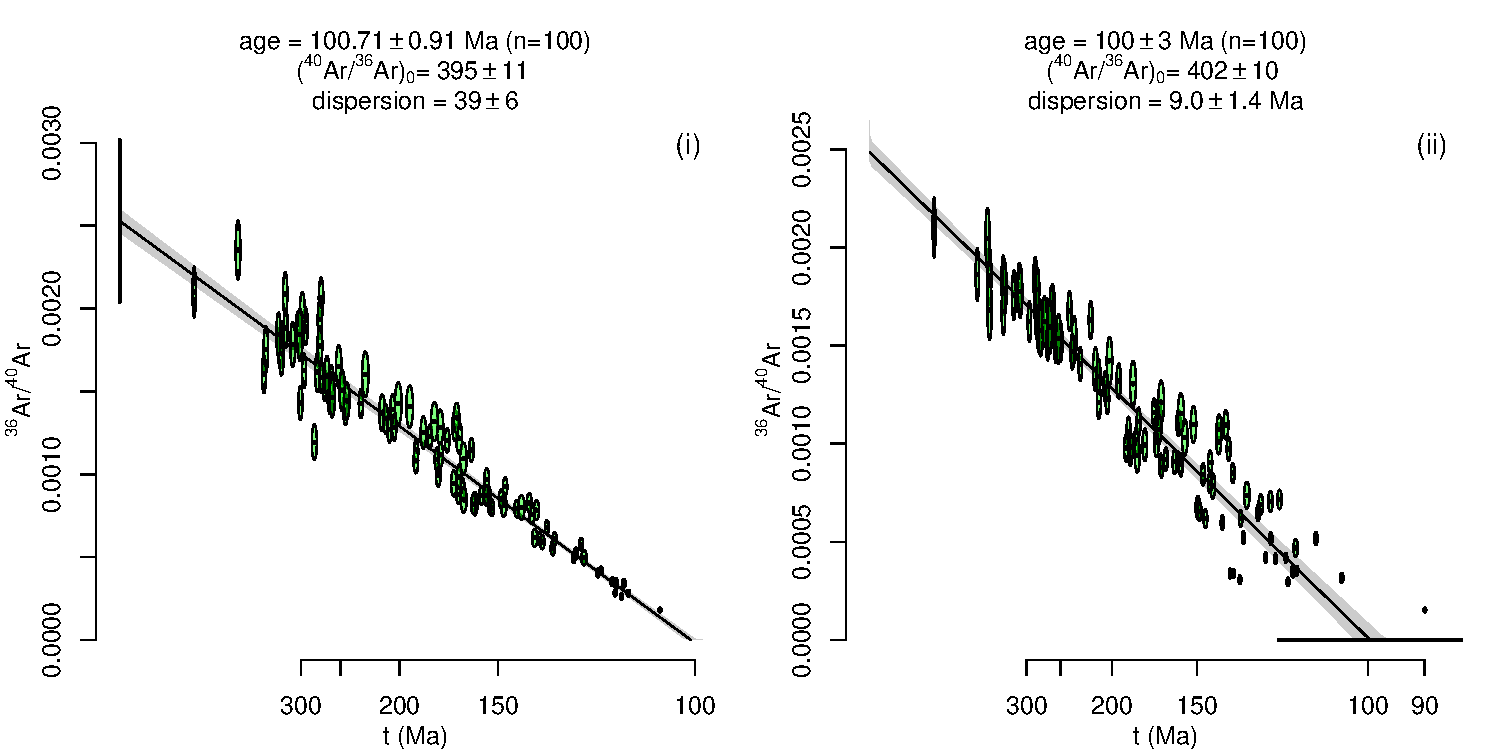
\includegraphics[width=15cm]{fig2.pdf}
  \caption{Model-3 regression of two synthetic Ar--Ar datasets.  (i)
    model~3a regression through 100 randomly drawn aliquots from an
    isochron with a true non-radiogenic ${}^{40}$Ar/${}^{39}$Ar-ratio
    of $400\pm{40}$ ($1\sigma$) and a true age of $100$\,Ma; (2)
    model~3b regression through 100 aliquots from an isochron with a
    true non-radiogenic ${}^{40}$Ar/${}^{39}$Ar-ratio of $400$ and a
    true age of $100\pm{10}$\,Ma ($1\sigma$). Error bars on the y- and
    x-axis show the overdispersion at 95\% confidence.}
  \label{fig:ArAr}
\end{figure}

\section{Anchored isochron regression}\label{sec:anchor}

Anchored isochron regression requires just a trivial modification of
the maximum likelihood algorithm. It suffices to treat the anchored
parameter as data. For example, the slope and intercept of a model~1
isochron can be anchored by maximising
$\mathcal{LL}_1(a,\mathbf{x}|b,\mathbf{X},\mathbf{Y},\mathbf{\Sigma})$
and
$\mathcal{LL}_1(b,\mathbf{x}|a,\mathbf{X},\mathbf{Y},\mathbf{\Sigma})$,
respectively. Note that these calculations assume that the anchor is
known exactly. This is reflected in the zero uncertainties of the
nonradiogenic component Figures~\ref{fig:cluster}.ii and
\ref{fig:cluster}.v, and of the radiogenic components of
Figures~\ref{fig:cluster}.iii and \ref{fig:cluster}.vi. Such absolute
certainty is unrealistic in the noisy world of geology.
Section~\ref{sec:anchorerr} introduces two ways to formally account
for uncertainty in anchored isochron regression.

\section{Accounting for anchor uncertainty}\label{sec:anchorerr}

When assigning uncertainty to statistical parameters, it is important
to clearly define the meaning of this uncertainty. In the case of
anchored isochron regression, the uncertainty of the intercept or
slope can carry two meanings. For example, when the intercept of an
isochron is anchored at a value $\bar{a} \pm \sigma_{\bar{a}}$, this
can either mean that:

\begin{description}
\item{\textbf{model~1}:} the data are underlain by a single isochron
  whose intercept is only approximately known, with a most likely
  value of $\bar{a}$ and a precision (standard error) of
  $\sigma_{\bar{a}}$.
\item{\textbf{model~3}:} the data were drawn from a family of isochron
  lines whose intercepts follow a normal distribution with mean
  $\bar{a}$ and standard deviation $\sigma_{\bar{a}}$.
\end{description}

These two different approaches can be implemented by replacing the
log-likelihood functions of Equation~\ref{eq:specific} with
\begin{equation}
  \begin{array}{ll}
    \mbox{\textbf{model~1}:} &
    \mathcal{LL}_1(a,b,\mathbf{x}|\bar{a},\sigma_{\bar{a}},\mathbf{X},\mathbf{Y},\mathbf{\Sigma}) =
    \mbox{constant} +
    \mathcal{LL}_1(a,b,\mathbf{x}|\mathbf{X},\mathbf{Y},\mathbf{\Sigma}) -
    \frac{1}{2} \left(\frac{a-\bar{a}}{\sigma_{\bar{a}}}\right)^2 \\
    \mbox{\textbf{model~3}:} &
    \mathcal{LL}_{3a}(b,\mathbf{x}|\bar{a},\sigma_{\bar{a}},\mathbf{X},\mathbf{Y},\mathbf{\Sigma})
  \end{array}
  \label{eq:aerr}
\end{equation}

The equivalent expressions for anchored slopes with uncertainty are
\begin{equation}
  \begin{array}{ll}
    \mbox{\textbf{model~1}:} &
    \mathcal{LL}_1(a,b,\mathbf{x}|\bar{b},\sigma_{\bar{b}},\mathbf{X},\mathbf{Y},\mathbf{\Sigma}) =
    \mbox{constant} +
    \mathcal{LL}_1(a,b,\mathbf{x}|\mathbf{X},\mathbf{Y},\mathbf{\Sigma}) -
    \frac{1}{2} \left(\frac{b-\bar{b}}{\sigma_{\bar{b}}}\right)^2 \\
    \mbox{\textbf{model~3}:} &
    \mathcal{LL}_{3b}(a,\mathbf{x}|\bar{b},\sigma_{\bar{b}},\mathbf{X},\mathbf{Y},\mathbf{\Sigma})
  \end{array}
  \label{eq:berr}
\end{equation}

Note that model~1 treats the slope and intercept as unknowns, so their
maximum likelihood estimates generally do \emph{not} equal the
anchored values $\bar{a}$ and $\bar{b}$. However, the smaller
$\sigma_{\bar{a}}$ and $\sigma_{\bar{b}}$ are relative to $\bar{a}$
and $\bar{b}$, the closer that $\hat{a}$ and $\hat{b}$ are to
$\bar{a}$ and $\bar{b}$. In contrast, anchored model~3 regression
fixes the dispersion of the anchored parameters, so that
$\hat{\sigma}_{a}=\sigma_{\bar{a}}$ for anchored intercepts, whereas
$\hat{\sigma}_{b}=\sigma_{\bar{b}}$ for anchored slopes.\medskip

Figure~\ref{fig:anchored} applies the two approaches to the synthetic
dataset of Figure~\ref{fig:cluster}, using anchors of $[D/d]_0 = 1 \pm
0.05$ and $[D/P]^\ast = 1 \pm 0.05$ ($1\sigma$). As expected, models~1
and 3 produce slightly different outcomes, with model~1 resulting in
$[D/d]_0$- and $[D/P]^\ast$-estimates that are slightly different than
the anchored values, whereas model~3 reproduces the anchors
exactly. The model~3 fits produce more precise estimates for the
unanchored quantities.  This reflects the fact that some of the
uncertainty in the isochron is captured by the dispersion parameter,
which is absent from the model~1 fit.\medskip

Model~3 partitions the analytical and geological uncertainty between
the standard errors of $\hat{a}$ and $\hat{b}$ on the one hand, and
the dispersion parameter on the other hand. It is not easy to
visualise this partitioned uncertainty. Figure~\ref{fig:anchored} uses
a grey confidence envelope to show the analytical uncertainty, and
black error bars to visualise the geological dispersion. Together
these two items represent the total uncertainty budget.\medskip

It is, of course, also possible to treat the dispersion parameter as
an unknown by maximising
$\mathcal{LL}_{3a}(b,\sigma_{a},\mathbf{x}|\bar{a},\mathbf{X},\mathbf{Y},\mathbf{\Sigma})$
or
$\mathcal{LL}_{3b}(a,\sigma_{b},\mathbf{x}|\bar{b},\mathbf{X},\mathbf{Y},\mathbf{\Sigma})$.
Section~\ref{sec:UPb} will give an example of this in the context of
U--Pb geochronology.

\begin{figure}[!ht]
  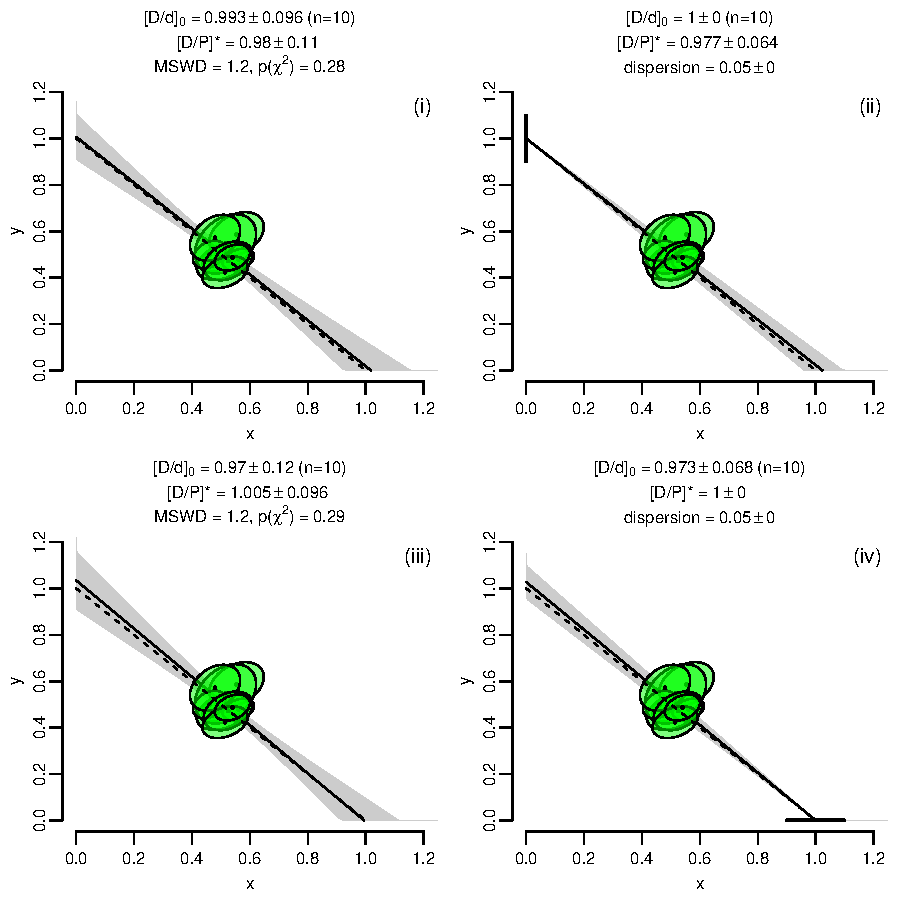
\includegraphics[width=11cm]{fig3.pdf}
  \caption{Anchored isochrons for the data of
    Figure~\ref{fig:cluster}, shown on inverse isochrons. Panels~i and
    ii anchor the non-radiogenic endmember composition to $[D/d]_0 = 1
    \pm 0.05$ (1$\sigma$).  Panels~iii and iv anchor the radiogenic
    endmember composition to $[D/P]^\ast = 1 \pm 0.05$ (1$\sigma$).
    Panels~i and iii use model~1 isochron regression, whereas panels
    ii and iv use model~3. Note how the estimated values for $[D/d]_0$
    and $[D/P]^\ast$ are exactly the same as the anchored values for
    model~3, but not for model~1. The vertical error bar in panel~ii
    and the horizontal error bar on panel~iv represent the fixed
    dispersion of the vertical and horizontal intercept,
    respectively.}
  \label{fig:anchored}
\end{figure}

\section{Pb/Pb isochrons}\label{sec:PbPb}

The ${}^{207}$Pb/${}^{206}$Pb-method is based on the paired decay of
two radioactive parents $P_1$ and $P_2$ (${}^{238}$U and ${}^{235}$U)
to two daughters $D_1$ and $D_2$ (${}^{206}$Pb and ${}^{207}$Pb,
respectively) in the presence of a non-radiogenic sister isotope $d$
(${}^{204}$Pb). This gives rise to the following implicit age
equation:
\begin{equation}
  \frac{[D_2/d]_i-[D_2/d]_0}{[D_1/d]_i-[D_1/d]_0} =
  \left[\frac{P_2}{P_1}\right]
  \frac{e^{\lambda_2t}-1}{e^{\lambda_1t}-1}
  \label{eq:tPbPb}
\end{equation}

\noindent where $\lambda_1$ and $\lambda_2$ are the decay constants of
$P_1$ and $P_2$, respectively, and $[P_2/P_1]$ is
constant. Equation~\ref{eq:tPbPb} can be recast into the generic form
of Equation~\ref{eq:yabx} to form a `D/D-isochron' using the mapping
of Table~\ref{tab:PDDD}. This gives rise to conventional
(${}^{207}$Pb/${}^{204}$Pb vs. ${}^{206}$Pb/${}^{204}$Pb) and inverse
(${}^{207}$Pb/${}^{206}$Pb vs. ${}^{204}$Pb/${}^{206}$Pb) isochrons.\medskip

Unlike inverse P/D-isochrons, which are characterised by negative
slopes, inverse D/D-isochrons have positive slopes. There is a perfect
symmetry between conventional and inverse D/D-isochrons in the sense
that the intercept of a conventional isochron equals the slope of an
inverse isochron and \emph{vice versa}.  This slightly changes and, in
fact, simplifies the procedure for anchored isochron
regression.\medskip

There is no need for flipped isochron regression of Pb/Pb
data. Instead, all possible scenarios can be handled by
straightforward model~1 and model~3a regression. Isochrons can be
anchored to the nonradiogenic component in conventional isochron
space, and to the radiogenic component in inverse isochron space.

\section{U/Pb isochrons}\label{sec:UPb}

The U/Pb method, like the Pb/Pb method, is based on the paired decay
of ${}^{238}$U to ${}^{206}$Pb and of ${}^{235}$U to ${}^{207}$Pb. The
two chronometers can be treated separately and plotted as
P/D-isochrons.  These two-dimensional isochrons can be anchored to the
radiogenic and nonradiogenic composition using the methods described
in Sections~\ref{sec:MLyork}--\ref{sec:anchorerr}.
\begin{equation}
  \begin{cases}
    \left[\frac{{}^{206}\mbox{Pb}}{{}^{204}\mbox{Pb}}\right]_i =
    \left[\frac{{}^{206}\mbox{Pb}}{{}^{204}\mbox{Pb}}\right]_0 +
    \left[\frac{{}^{238}\mbox{U}}{{}^{204}\mbox{Pb}}\right]_i
    \left(e^{\lambda_{238}t}-1\right)\\
    \left[\frac{{}^{207}\mbox{Pb}}{{}^{204}\mbox{Pb}}\right]_i =
    \left[\frac{{}^{207}\mbox{Pb}}{{}^{204}\mbox{Pb}}\right]_0 +
    \left[\frac{{}^{235}\mbox{U}}{{}^{204}\mbox{Pb}}\right]_i
    \left(e^{\lambda_{235}t}-1\right)\\
  \end{cases}
\end{equation}

Alternatively, the two ingrowth equations can also be coupled, forming
a three dimensional `total-Pb/U isochron'. This problem can be solved
using the method of maximum likelihood \citep{ludwig1998}. There is
just one important difference between this solution and the York-like
algorithm of Section~\ref{sec:MLyork}. York regression is formulated
in terms of a generic intercept ($a$) and slope ($b$). In contrast,
the `Ludwig' algorithm is formulated in terms of the actual
non-radiogenic $^{206}$Pb/$^{204}$Pb ($=\alpha$) and
$^{207}$Pb/$^{204}$Pb (=$\beta$) ratio, as well as the age ($t$) of
the system.\medskip

It is relatively straightforward to generalise the concept of model~3
regression to total-Pb/U isochrons when the dispersion is attributed
to the isochron age. However, it is not immediately clear how to do the
same for the nonradiogenic composition, because this would require
partitioning the dispersion between the $\alpha$- and
$\beta$-parameters. This paper will not attempt to answer this
question. Instead, let us conclude the technical discussion by
shifting to a far more common type of U/Pb data.\medskip

Most published U/Pb studies do not report $^{204}$Pb because this
nuclide is rare and difficult to measure. Instead, `semitotal-Pb/U'
regression is done in Wetherill or Tera-Wasserburg concordia space,
which are akin to conventional and inverse isochron space,
respectively. In the absence of a nonradiogenic sister isotope of Pb,
the isochron is then redefined as as a mixing line between an
inherited ${}^{207}$Pb/${}^{206}$Pb-ratio and the radiogenic
${}^{206}$Pb/${}^{238}$U- and ${}^{207}$Pb/${}^{235}$U-ratios.\medskip

The semitotal-Pb/U problem can be cast into a maximum likelihood
format by replacing Equation~\ref{eq:model1} with
\begin{equation}
  \begin{cases}
    X_i = x_i + e^{\lambda_{235}t} - 1 + \epsilon_{x,i} \\
    Y_i = a + b x_i + \epsilon_{y,i}
  \end{cases}
  \label{eq:UPb}
\end{equation}

\noindent where $X_i$ and $Y_i$ are the measured
${}^{207}$Pb/${}^{235}$U- and ${}^{206}$Pb/${}^{238}$U-ratios of the
$i$\textsuperscript{th} aliquot, respectively; $x_i$ is the true
${}^{207}$Pb$_0/{}^{235}$U-ratio of the $i$\textsuperscript{th}
aliquot; $a = e^{\lambda_{238}t}-1$ and
$b = [{}^{206}\mbox{Pb}/{}^{207}\mbox{Pb}]_0[{}^{235}\mbox{U}/{}^{238}\mbox{U}]$.
Equation~\ref{eq:UPb} can be solved using the same recipe as the York
reformulation of Sections~\ref{sec:MLyork}--\ref{sec:anchorerr}, with
the caveat that the isochron terminates on the concordia line at the U/Pb
composition corresponding to $t$.\medskip

Figure~\ref{fig:UPb} shows a model~3a anchored semitotal-Pb/U isochron
in Tera-Wasserburg space. The true age for this synthetic dataset is
1500~Ma. The unconstrained model~1 isochron produces an imprecise
isochron age of $1491\pm{100}$~Ma, which is improved to
$1504\pm{38}$~Ma by anchoring to
$[{}^{207}\mbox{Pb}/{}^{206}\mbox{Pb}]_0=1.1$. Just like the
P/D-isochrons of Figure~\ref{fig:anchored}, the uncertainty budget for
the U/Pb-isochrons of Figure~\ref{fig:UPb} is partitioned between the
analytical and geological dispersion, where the latter is treated as a
free parameter with a maximum likelihood estimate of
$\hat{\sigma}_a={0.053}\pm{0.026}$.

\begin{figure}[!ht]
  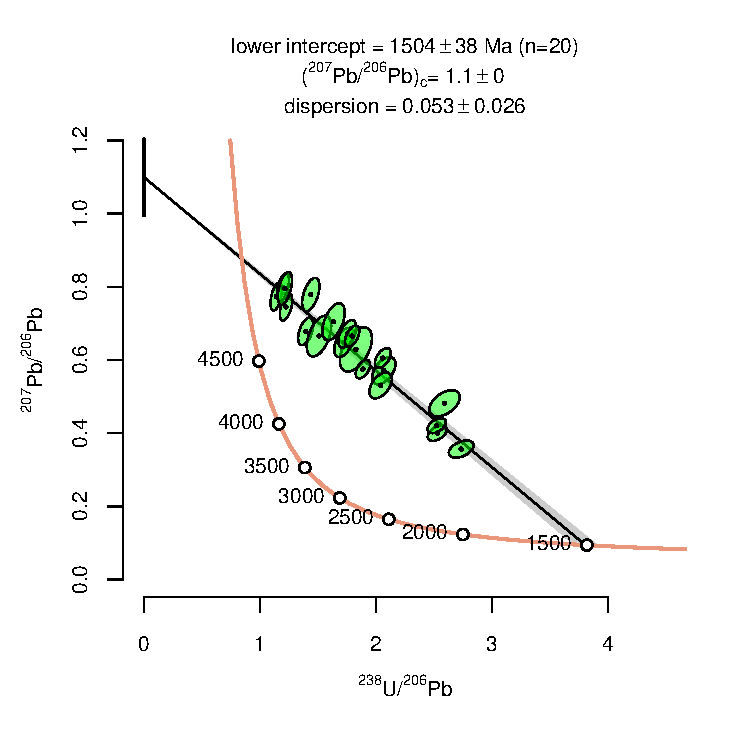
\includegraphics[width=8cm]{fig4.pdf}
  \caption{Model~3a semitotal-Pb/U isochron for a synthetic dataset
    with a true age $t=1500$~Ma, anchored to $^{207}$Pb/$^{206}$Pb$=
    1.10$ with the dispersion parameter treated as a free
    parameter.}
  \label{fig:UPb}
\end{figure}

\section{Implementation in \texttt{IsoplotR}}\label{sec:IsoplotR}

All the algorithms presented in this paper have been implemented in
the free and open geochronological toolbox IsoplotR
\citep{vermeesch2018c}. The ability to fit isochrons with models~1, 2
and 3 dates back to IsoplotR's first public release. Versions~2.1 and
5.2 added model~1 anchors to U/Pb ischrons without and with
uncertainty, respectively. Anchored York regression and model~3
anchors with uncertainty were added to IsoplotR 6.0. These funtions
can be accessed via the GUI or from the command line.\medskip

In the GUI, anchored regression is available from the `isochron' menu
(so not from the `concordia' menu for U/Pb data). The relevant
settings can be selected from the `Options' menu and should be self
explanatory. Using a built-in ${}^{40}$Ar/${}^{39}$Ar-dataset to
illustrate the command-line functionality, and starting with an
unanchored inverse isochron fit using York regression:

\begin{verbatim}
library(IsoplotR)
attach(examples)
isochron(ArAr)
\end{verbatim}

To carry out model~3a isochron regression anchored to a variable
initial ${}^{40}$Ar/${}^{36}$Ar-ratio of $300\pm{5}$ (1$\sigma$):

\begin{verbatim}
settings('iratio','Ar40Ar36',300,5)
isochron(ArAr,anchor=1,model=3,taxis=TRUE)
\end{verbatim}

\noindent where \texttt{settings($\ldots$)} is used to change the
atmospheric argon composition, \texttt{anchor=1} fixes the isochron to
the inherited component, \texttt{model=3} tells IsoplotR to assign the
dispersion to the reported uncertainty of the atmospheric
${}^{40}$Ar/${}^{36}$Ar-ratio, and \texttt{taxis=TRUE} changes the
x-axis to a time scale (as in Figure~\ref{fig:ArAr}).\medskip

Finally, to carry out model~3b isochron regression anchored to a
radiogenic composition that was set at $62\pm{1}~$Ma~($1\sigma$):

\begin{verbatim}
isochron(ArAr,anchor=c(2,62,1),model=3,taxis=TRUE)
\end{verbatim}

The dispersion can be changed to a free parameter by setting the third
element of the \texttt{anchor} argument to a non-positive
value. Documentation for additional options and settings can be
accessed from the console, using the \verb|help(isochron)| or
\verb|?isochron| commands.

\section{Conclusions}\label{sec:conclusions}

This paper builds on previous work by \citet{mcintyre1966},
\citet{titterington1979} and \citet{ludwig2003}. \citet{mcintyre1966}
introduced the concept of model~3 isochron regression, attributing the
excess dispersion of errorchrons to variability of the inherited
component. This approach is implemented in Isoplot \citep{ludwig2003}
and is referred to as model~3a regression in this paper. Note that
\citet{mcintyre1966}'s definition of model~2 regression differs from
that of \citet{ludwig2003}. It is more akin (but not identical) to the
$\sqrt{\mbox{MSWD}}$ approach of
Section~\ref{sec:overdispersion}.\medskip

\citet{titterington1979} recast the model~3 algorithm of
\citet{mcintyre1966} in a maximum likelihood framework. This paper
extends the maximum likelihood approach to a second type of geological
scenario, in which excess dispersion of the data around the isochron
is not attributed to the inherited component but to the radiogenic
component. This approach is referred to as model~3b
regression.\medskip

The maximum likelihood formulation of isochron regression can also be
used to anchor isochrons to either the inherited or the radiogenic
component, and to assign geologically meaningful uncertainty to the
anchor. In reality it is possible that some samples are affected by
both mechanisms, so that different aliquots of the same sample differ
in their initial ratios as well as the timing of their isotopic
closure. Unfortunately, it is not possible to simultaneously capture
both types of dispersion using the algorithms of this paper.\medskip

The difference between model~1 and model~3 regression represents two
contrasting views of geological reality. The model~1 approach assumes
that the isotopic composition of minerals represents discrete
components recorded at distinct events. In contrast, model~3 isochrons
represent a `fuzzier' reality, in which the initial composition or
timing of isotopic closure are allowed to vary within a rock. Under
the latter model, the concept of an `errorchron' no longer makes
sense.

\section*{Code availability}

IsoplotR is available from CRAN
(\url{https://CRAN.R\-project.org/package=IsoplotR}) and GitHub
(\url{https://github.com/pvermees/IsoplotR})


\appendix

\section{Definitions}\label{app:definitions}

\begin{description}
\item{$P$:} a radioactive parent (e.g., ${}^{87}$Rb).
\item{$D$:} the radiogenic daughter of $P$ (e.g., ${}^{87}$Sr).
\item{$d$:} a non-radiogenic sister isotope of $D$ (e.g., ${}^{86}$Sr).
\item{$a$, $b$, $x_i$, $y_i$:} the true (but unknown) values of the
  intercept, slope and isotopic ratio of the $i$\textsuperscript{th}
  aliquot (out of $n$ aliquots) from a sample.
\item{$\hat{a}$, $\hat{b}$, $\hat{x}_i$, $\hat{y}_i$:} the estimated
  values of $a$, $b$, $x_i$ and $y_i$, respectively.
\item{$X_i$, $Y_i$:} the measured values of $x_i$ and $y_i$,
  respectively.
\item{$s[X_i]$, $s[Y_i]$, $s[X_i,Y_i]$:} the standard errors and
  covariance of $X_i$ and $Y_i$.
\item{$\epsilon_{x,i}=X_i-x_i$, $\epsilon_{y,i}=Y_i-y_i$:} the
  residuals of the data around the best fit line.
\item{$\mathbf{\Sigma}_i$:} the ${2}\times{2}$ covariance matrix of $X_i$ and $Y_i$
\item{$\mathbf{x}$, $\mathbf{y}$, $\mathbf{X}$, $\mathbf{Y}$,
  $\mathbf{\Sigma}$:} arrays and sets containing all $n$ $x_i$, $y_i$,
  $X_i$, $Y_i$ and $\mathbf{\Sigma}_i$-values.
\end{description}

All uncertainties in this paper are reported as 95\% confidence
intervals except if noted otherwise.

\begin{table}[!ht]
  \centering
  \caption{Assignment of the isotopic ratios for P/D- and
    D/D-isochrons to the generic parameters of
    Equation~\ref{eq:yabx}.}
  \label{tab:PDDD}
  \begin{tabular}{ccccc}
    ~ & \multicolumn{2}{c}{P/D} & \multicolumn{2}{c}{D/D} \\ \cline{2-5}
    parameter & conventional & inverse & conventional & inverse \\ \hline
    $x_i$ & $[P/d]_i$ & $[P/D]_i$ & $[D_1/d]_i$ & $[d/D_1]_i$ \\
    $y_i$ & $[D/d]_i$ & $[d/D]_i$ & $[D_2/d]_i$ & $[D_2/D_1]_i$ \\
    $a$ & $[D/d]_0$ & $[d/D]_0$ & $[D_2/d]_0$ & $[D_2/D_1]^\ast$ \\
    $b$ & $[D/P]^\ast$ & $-[d/D]_0/[P/D]^\ast$ & $[D_2/D_1]^\ast$ & $[D_2/d]_0$ \\ \hline
  \end{tabular}
\end{table}

\section{Data}\label{app:syntheticdata}

The synthetic data of Figures~\ref{fig:cluster} and \ref{fig:anchored}
were generated as follows:
\begin{enumerate}
\item Generate $\mathbf{x}$ by drawing ten random numbers from a
  logit-normal distribution where the mean and standard deviation of
  the logits are 0 and 1/5, respectively.\label{it:logit}
\item Generate $\mathbf{y}$ by plugging $\mathbf{x}$ into
  Equation~\ref{eq:yabx} with $a=b=1$.\label{it:xab2y}
\item Turn the resulting ten pairs of $\{x_i,y_i\}$-values into ten
  trios of $\{P_i,D_i,d_i\}$-values where $d_i$ is a random number
  between 100 and 500.\label{it:xy2PDd}
\item Use each of the $\{P_i,D_i,d_i\}$-values obtained in the
  previous step as parameters for a Poisson experiment.
\item Use the Poisson values obtained in the previous step to form ten
  pairs of $\mathbf{X}$- and $\mathbf{Y}$-measurements and their
  (correlated) uncertainties.\label{it:PoisXY}
\item Add some excess dispersion by shrinking the uncertainties by
  20\%.
\end{enumerate}

Note that this procedure fits the definition of a model~1 isochron,
even though panels (ii) and (iv) of Figure~\ref{fig:anchored} use the
resulting data to illustrate model~3 regression. The synthetic data of
Figures~\ref{fig:ArAr} and \ref{fig:UPb} are generated using a
slightly different algorithm that simulates model~3a and 3b
overdispersion. This modified procedure uses steps~\ref{it:logit} and
\ref{it:xy2PDd}--\ref{it:PoisXY} of the procedure for
Figure~\ref{fig:cluster} whilst replacing step~\ref{it:xab2y} with a
random effects model, in which $a$ and $b$ are drawn from random normal
distributions with standard deviations corresponding to the dispersion
parameter $\sigma_{\bar{a}}$ (10\% for Figure~\ref{fig:ArAr}.i and 5\%
for Figure~\ref{fig:UPb}) and $\sigma_{\bar{b}}$ (10\% for
Figure~\ref{fig:ArAr}.ii).

\section{Testing overdispersion}\label{app:X2}

Whether a dataset is overdispersed with respect to the analytical
uncertainties can be formally assessed using the Chi-statistic and
test. To this end, calculate the $\chi^2$-statistic using the sum of
squares term of Equation~\ref{eq:LL}.
\begin{equation}
  \chi^2 = \sum\limits_{i=1}^{n} \mathbf{\Delta}_i^T \mathbf{\Sigma}_i^{-1} \mathbf{\Delta}_i
  \label{eq:X2}
\end{equation}

If analytical uncertainty is the only source of dispersion in the
dataset, then $\chi^2$ is expected to follow a Chi-square distribution
with $df=n-2$ (or, for anchored regression, $df=n-1$) degrees of
freedom.  This is called the `null distribution'. The probability of
observing a value greater than $\chi^2$ under this distribution is
called the p-value. A p-value cutoff of 0.05 is generally used to
distinguish isochrons ($p\geq{0.05}$) from errorchrons
($p<0.05$). Dividing Equation~\ref{eq:X2} by the number of degrees of
freedom ($df$) produces a `reduced Chi-square statistic', which is
known to geologists as an MSWD \citep{mcintyre1966}:
\begin{equation}
  \mbox{MSWD} = \frac{\chi^2}{df}
  \label{eq:MSWD}
\end{equation}

In the absence of overdispersion, and for sufficiently large samples
($n>20$), the expected null distribution of the MSWD is approximately
normal with a mean of 1 and a standard deviation $\sqrt{2/df}$
\citep{wendt1991}. This information can be used as an alternative
way to test the null hypothesis.

\section{Further details about the maximum likelihood solution}\label{app:algorithm}

Section~\ref{sec:specific} described how the log-likelihood functions
of Equation~\ref{eq:specific} can be maximised in a two step process:
(1) find the $x_i$-values that maximise $\mathcal{LL}$ for any pair of
$a$- and $b$-values, and (2) search the space of $a$- and $b$- values
until the overall maximum is found. For model~1 regression, the first
step has a direct solution. Introducing some shorthand notation for
the inverse of the covariance matrix $\Sigma_i$:
\begin{equation}
  \mathbf{\Sigma}_i^{-1} 
  \equiv
  \left[
  \begin{array}{@{}cc@{}}
    \Omega_{1,1}^i & \Omega_{1,2}^i\\
    \Omega_{2,1}^i & \Omega_{2,2}^i
  \end{array}
  \right],
\end{equation}

\noindent where $\Omega_{1,2}=\Omega_{2,1}$. The fitted points $x_i$
can be found by solving:
\begin{equation}
  \left.\frac{\partial\mathcal{LL}_1}{\partial{x_i}}\right|_{\hat{x}_i} = 0
\end{equation}

\noindent which yields
\begin{equation}
  \hat{x}_i =
  \frac{X_i(\Omega_{1,1}^i + b \Omega_{1,2}^i) + (Y_i-a)(\Omega_{2,1}^i+b\Omega_{2,2}^i)}
       {(\Omega_{1,1}^i + b \Omega_{1,2}^i) + b(\Omega_{2,1}^i+b\Omega_{2,2}^i)}.
       \label{eq:xi}
\end{equation}

The same approach can be used for model~3a regression (with
$\partial{\mathcal{LL}_{3a}|}/\partial{x_i}=0$). However, it does not
work for model~3b isochrons because
$\partial^2{\mathcal{LL}_{3b}}/\partial{x_i}\partial{x_j}\neq{0}$ when
${i}\neq{j}$. Therefore, the $x_i$s are interdependent and cannot be
solved separately. Although it is possible to jointly optimise the
entire $\mathbf{x}$-vector, this takes considerably longer than
model~1 and model~3a regression.  Fortunately, as explained in
Section~\ref{sec:flipper}, model~3b regression can be reformulated in
terms of the model~3a algorithm.

%\appendixfigures  %% needs to be added in front of appendix figures

%\appendixtables   %% needs to be added in front of appendix tables

%% Please add \clearpage between each table and/or figure. Further guidelines on figures and tables can be found below.

\section*{Author contribution}

PV is sole author of this contribution

\section*{Competing interests}

PV is an Associate Editor of this journal

\section*{Acknowledgements}

The author would like to thank reviewers Donald Davis and John Rudge
for suggesting to expand the discussion of model-3 regression, and for
checking the equations. This work was completed during a sabbatical
stay at the Institute of Geology and Geophysics, Chinese Academy of
Sciences, which was supported by CAS' President's International
Fellowship Initiative (PIFI). The author would like to thank Xian-Hua
Li of IGG-CAS and Yang Li of Peking University for hosting him at
IGG-CAS.  He would also like to thank IsoplotR users Guilhem Hoareau
(CNRS, France), Shitou Wu (IGG-CAS, China) and Stijn Glorie (Adelaide,
Australia) for discussing the utility of anchored isochrons, and
moving this feature up the priority list for IsoplotR.

%\bibliographystyle{/home/pvermees/Dropbox/anchor/copernicus.bst}
%\bibliography{/home/pvermees/Dropbox/biblio.bib}

\begin{thebibliography}{10}
\providecommand{\natexlab}[1]{#1}
\providecommand{\url}[1]{\texttt{#1}}
\providecommand{\urlprefix}{}
\expandafter\ifx\csname urlstyle\endcsname\relax
  \providecommand{\doi}[1]{https://doi.org/\discretionary{}{}{}#1}\else
  \providecommand{\doi}{https://doi.org/\discretionary{}{}{}\begingroup
  \urlstyle{rm}\Url}\fi

\bibitem[{Da{\"e}ron and Vermeesch(2023)}]{daeron2023}
Da{\"e}ron, M. and Vermeesch, P.: {Omnivariant generalized least squares
  regression: Theory, geochronological applications, and making the case for
  reconciled $\Delta_{47}$ calibratibons}, Chemical Geology, p. 121881, 2023.

\bibitem[{Li and Vermeesch(2021)}]{li2021}
Li, Y. and Vermeesch, P.: Inverse isochron regression for Re--Os, K--Ca and
  other chronometers, Geochronology, 3, 415--420, 2021.

\bibitem[{{Ludwig}(1998)}]{ludwig1998}
{Ludwig}, K.~R.: {On the treatment of concordant uranium-lead ages}, Geochimica
  et Cosmochimica Acta, 62, 665--676, \doi{10.1016/S0016-7037(98)00059-3},
  1998.

\bibitem[{Ludwig(2003)}]{ludwig2003}
Ludwig, K.~R.: {User's manual for Isoplot 3.00: a geochronological toolkit for
  Microsoft Excel}, Berkeley Geochronology Center Special Publication, 4, 2003.

\bibitem[{{McIntyre} et~al.(1966){McIntyre}, {Brooks}, {Compston}, and
  {Turek}}]{mcintyre1966}
{McIntyre}, G.~A., {Brooks}, C., {Compston}, W., and {Turek}, A.: {The
  Statistical Assessment of Rb-Sr Isochrons}, Journal of Geophysical Research,
  71, 5459--5468, 1966.

\bibitem[{Schaen et~al.(2021)Schaen, Jicha, Hodges, Vermeesch, Stelten, Mercer,
  Phillips, Rivera, Jourdan, Matchan et~al.}]{schaen2021}
Schaen, A.~J., Jicha, B.~R., Hodges, K.~V., Vermeesch, P., Stelten, M.~E.,
  Mercer, C.~M., Phillips, D., Rivera, T.~A., Jourdan, F., Matchan, E.~L.,
  et~al.: Interpreting and reporting $^{40}$Ar/$^{39}$Ar geochronologic data,
  Bulletin, 133, 461--487, 2021.

\bibitem[{Titterington and Halliday(1979)}]{titterington1979}
Titterington, D.~M. and Halliday, A.~N.: On the fitting of parallel isochrons
  and the method of maximum likelihood, Chemical Geology, 26, 183--195, 1979.

\bibitem[{Vermeesch(2018)}]{vermeesch2018c}
Vermeesch, P.: {\texttt{IsoplotR}: a free and open toolbox for geochronology},
  Geoscience Frontiers, 9, 1479--1493, 2018.

\bibitem[{Wendt and Carl(1991)}]{wendt1991}
Wendt, I. and Carl, C.: The statistical distribution of the mean squared
  weighted deviation, Chemical Geology: Isotope Geoscience Section, 86,
  275--285, 1991.

\bibitem[{York et~al.(2004)York, Evensen, Mart\'{i}nez, and
  De~Basabe~Delgado}]{york2004}
York, D., Evensen, N.~M., Mart\'{i}nez, M.~L., and De~Basabe~Delgado, J.:
  {Unified equations for the slope, intercept, and standard errors of the best
  straight line}, American Journal of Physics, 72, 367--375, 2004.

\end{thebibliography}


\end{document}
